% =====================================================================
%  Optimizing Input Representations for Word-in-Context:
%  A Controlled Ablation Study
%  Springer LNCS/LNAI format  --  AIxIA 2026 submission
%
%  Requires: llncs.cls (Springer).
%
%  Figures expected in the project root:
%    ablation_plot_cv_300dpi.png   (main 5-fold CV bar chart, Fig. 1, Sec. 4.1)
%    factorial_contrasts.pdf       (forest plot of contrasts, Fig. 2, Sec. 4.2)
%    prefix_decomposition.pdf      (RoBERTa decomposition, Fig. 3, Sec. 4.2)
% =====================================================================
\documentclass[runningheads]{llncs}

\usepackage{graphicx}
\usepackage{booktabs}
\usepackage{multirow}
\usepackage{amsmath}
\usepackage{amssymb}
\usepackage{array}
\usepackage[T1]{fontenc}
\usepackage{url}
% protrusion-only keeps the layout clean in every TeX setup; on Overleaf you may
% switch to \usepackage{microtype} (adds font expansion) for marginally tighter spacing.
\usepackage[protrusion=true,expansion=false]{microtype}
% Let TeX absorb the last few points of over-long lines instead of spilling
% into the margin; content is unchanged, only interword spacing flexes slightly.
\setlength{\emergencystretch}{1.5em}
% Float placement: allow LaTeX to pack more of each page with floats before
% starting a float-only page. Content is unchanged; only placement is affected.
\renewcommand{\topfraction}{0.9}
\renewcommand{\bottomfraction}{0.7}
\renewcommand{\textfraction}{0.1}
\renewcommand{\floatpagefraction}{0.8}

\begin{document}

\title{Optimizing Input Representations for Word-in-Context:
A Controlled Ablation Study}

\titlerunning{Input Ablation for Word-in-Context}

% NOTE: the running head "C. Daloiso et al." is the standard LNCS author
% running head required by Springer; do not remove \authorrunning.
\author{Claudio Daloiso\inst{1} \and
Francesca Fallucchi\inst{1} \and
Manuel Gozzi\inst{1} \and
Alessandro Ligi\inst{1}}
% ORCID: add \orcidID{...} after each author name if available.

\authorrunning{C. Daloiso et al.}

\institute{Department of Engineering Sciences, Guglielmo Marconi University,\\
00193 Rome, Italy\\
\email{c.daloiso@studenti.unimarconi.it, f.fallucchi@unimarconi.it,}\\
\email{m.gozzi@studenti.unimarconi.it, a.ligi@unimarconi.it}}

\maketitle

\begin{abstract}
The Word-in-Context (WiC) task requires deciding whether a target word carries
the same meaning in two different sentential contexts. When fine-tuning
Transformer encoders, a common and intuitive choice is to mark the target word
with special tokens, on the assumption that this helps the model locate the
relevant span. We test that assumption with a controlled $2 \times 2$ factorial
ablation on SuperGLUE WiC, separating explicit target-span marking (span
highlighting) from a lexical prefix that prepends the target word, and decompose
the prefix to isolate the lemma from the part-of-speech (POS) tag. The design is
evaluated on DeBERTa-large and RoBERTa-large with 5-fold cross-validation on the
union of training and development splits ($N = 6066$), using McNemar's test,
Holm--Bonferroni correction and bootstrap confidence intervals. Span
highlighting provides no benefit and significantly degrades DeBERTa-large
(removing the markers improves out-of-fold accuracy by $2.26$~pp,
$p_{\text{Holm}} < 0.001$), consistent with prior observations in relation
extraction that in-vocabulary markers can match or outperform newly introduced
special tokens. The lexical prefix significantly improves both backbones when
markers are absent. Since the SuperGLUE WiC release exposes no usable POS field,
the decomposition contrasts the target lemma against a constant control, and on
RoBERTa-large the lemma is the active component. The contribution is a
controlled, statistically grounded quantification of input-formatting choices
frequently adopted without separate verification.

\keywords{Word-in-Context \and Transformer Encoders \and Span Highlighting
\and Ablation Study \and Natural Language Processing}
\end{abstract}

% =====================================================================
\section{Introduction}
\label{sec:intro}

Word-sense discrimination is a long-standing problem in computational
linguistics: a word may take on different meanings depending on its context.
The distributional view of meaning, summarised by Firth's dictum that one shall
know a word by the company it keeps~\cite{firth1957synopsis}, holds that the
surrounding context rather than the word form in isolation determines the
intended sense. The Word-in-Context (WiC)
dataset operationalises this view as a binary task: given two sentences and a
shared target word, a model must decide whether the word carries the same
meaning in both contexts~\cite{pilehvar2019wic}. WiC was subsequently
incorporated into SuperGLUE~\cite{wang2019superglue}.

With the rise of Transformer encoders such as BERT, RoBERTa, and
DeBERTa~\cite{devlin2019bert,liu2019roberta,he2021deberta}, sentence-pair
classification tasks are typically addressed through supervised fine-tuning.
Beyond the choice of backbone, the way the input is represented can also
influence performance. A natural choice for WiC is to mark the target word with
special tokens, for example ``Do you want to come over to my
\texttt{<TW>}place\texttt{</TW>} later?'', on the intuition that explicit
markers help the model focus on the relevant span. This strategy (span
highlighting) is closely related to marking techniques used in relation
extraction and other semantic tasks. Yet the
special tokens are not part of the model's original pre-training distribution
and must be learned during fine-tuning; moreover, their effect can be conflated
with other signals such as a prefix prepending the target word. This motivates
the central question: does explicit span highlighting genuinely improve WiC, or
does the useful signal mainly come from a lexical prefix?

To answer this, we pose three research questions. First, does explicit span
highlighting improve WiC over an otherwise identical input, or is it unnecessary
or even harmful (RQ1)? Second, does a lexical prefix improve WiC, and does it
interact with span highlighting (RQ2)? Third, within the prefix, is the active
component the target lemma or the part-of-speech tag (RQ3)?

We address these questions with a $2 \times 2$ factorial ablation that separates
span marking from the lexical prefix, and further decompose the prefix into its
lemma and part-of-speech components. Throughout, the architecture is held
constant by design: every condition uses the same backbone and the same standard
sequence-classification head, so only the surface form of the input varies. A
span-aware component---span pooling, a token-weighted loss, or an attention
bias---would alter model and input together and confound the contrast this study
isolates; such variants are a follow-up (Section~\ref{sec:conclusion}). Our
study contributes a controlled ablation
of target-span marking and a lexical prefix on SuperGLUE WiC, evaluated on
DeBERTa-large and RoBERTa-large under a frozen training configuration with
5-fold cross-validation on $N = 6066$ examples, together with a statistical
analysis based on McNemar's test, Holm--Bonferroni correction, and bootstrap
confidence intervals, and an error analysis of the headline effect.

Our main results are clear-cut. Span highlighting provides no benefit and
significantly degrades DeBERTa-large (a $2.26$~pp drop, $p_{\text{Holm}} <
0.001$), whereas the lexical prefix significantly improves both backbones when
markers are absent (up to $+2.18$~pp on RoBERTa-large). The target lemma, not
the part-of-speech tag, carries the signal, and the effect of the markers is
diffuse rather than concentrated on an identifiable subset.

The remainder of the paper is organised as follows.
Section~\ref{sec:related} reviews related work, Section~\ref{sec:method}
describes the data, input conditions, models and evaluation protocol, and
Section~\ref{sec:results} reports the per-condition results, the statistical
analysis and the error analysis. Sections~\ref{sec:discussion},
\ref{sec:limitations} and~\ref{sec:conclusion} discuss the findings, state the
limitations and conclude.

% =====================================================================
\section{Related Work}
\label{sec:related}

WiC was introduced by Pilehvar and Camacho-Collados as a benchmark for
context-sensitive representations of word meaning~\cite{pilehvar2019wic}, and
included in SuperGLUE as a challenging test of contextual lexical
discrimination~\cite{wang2019superglue}. A relevant caveat for any input-side
study is that WiC does not test context and target word symmetrically: Liu et
al.~\cite{liu2021context} probe lexical-semantic datasets with masked inputs and
find that WiC-style tasks exhibit a strong context bias, with models able to
exploit dataset regularities. This matters for our work, because it means that a
lexical anchor on the target word is not trivially expected to help, and that
any benefit deserves explicit measurement rather than assumption.

These tasks are typically addressed by fine-tuning Transformer encoders: BERT
introduced bidirectional pre-training with masked language
modeling~\cite{devlin2019bert}, RoBERTa improved the pre-training
procedure~\cite{liu2019roberta}, and DeBERTa introduced disentangled attention
between content and position~\cite{he2021deberta}. In WiC these models are used
as cross-encoders, where the two sentences are concatenated and the target word
is not automatically privileged, which motivates explicit localization or
lexical signals.

Marking the target span is a familiar device in adjacent tasks. In relation
extraction, \emph{Matching the Blanks} demonstrated that entity-centric
representations based on marked spans are effective~\cite{soares2019matching},
and, more directly relevant to our question, Zhou and
Chen~\cite{zhou2022improved} systematically compare marking variants and
distinguish between markers that introduce \emph{new special tokens} and markers
that reuse \emph{in-vocabulary punctuation}; the punctuation-based variant, which
adds no out-of-distribution tokens, is a strong baseline. This distinction
directly anticipates our finding for WiC: when a marker is realised through
tokens that the model has never seen in pre-training, the benefit of marking is
not guaranteed. Within WiC and adjacent tasks, XL-LEXEME highlights the target
word in a bi-encoder for lexical semantic change~\cite{cassotti2023xllexeme}, and
participants in the MCL-WiC shared task used signals on the target word in
multilingual settings~\cite{martelli2021mclwic,gupta2021mcliitk}; crucially,
these systems \emph{assume} highlighting to be beneficial and do not evaluate the
contribution of the marking against a baseline without it. Our ablation addresses
precisely this open question in the cross-encoder setting: the question is not
whether to mark the target, but whether marking is necessary when compared to a
simple lexical prefix. A related idea is the lexical anchor: GlossBERT prepends
WordNet gloss definitions to the input context for word sense
disambiguation~\cite{huang2019glossbert}, showing that an anchor placed before
the sentence can guide the model toward the relevant word; unlike the prefix
studied here, it relies on external sense inventories rather than the target
lemma alone.

Overall, prior work motivates our study but does not isolate the contribution of
span highlighting and lexical prefixing under a controlled protocol;
Table~\ref{tab:related} summarises this positioning. To the best of our
knowledge, no prior work jointly isolates span highlighting and a lexical prefix
in a $2 \times 2$ factorial ablation on SuperGLUE WiC, nor decomposes the prefix
into lemma and POS components. We do not claim to introduce target marking, nor
that newly initialized markers can underperform---an effect already documented
in relation extraction~\cite{zhou2022improved}; our contribution is to establish
it, under statistical control, in the WiC cross-encoder setting and to contrast
marking against a lexical prefix.

\begin{table}[t]
\centering
\caption{Representative prior work. Mark.\ = target/span marking; Pref.\ = lexical prefix; $2{\times}2$ = controlled factorial ablation.}
\label{tab:related}
\setlength{\tabcolsep}{3pt}
\footnotesize
\begin{tabular}{>{\raggedright\arraybackslash}p{2.05cm}>{\raggedright\arraybackslash}p{1.6cm}>{\raggedright\arraybackslash}p{1.7cm}ccc >{\raggedright\arraybackslash}p{3.15cm}}
\toprule
Work & Task & Method & Mark.\ & Pref.\ & $2{\times}2$ & Difference from our work\\
\midrule
WiC \cite{pilehvar2019wic} & WiC dataset & baselines & No & No & No & Defines the task; does not study input formatting.\\
SenseBERT \cite{levine2020sensebert} & WiC & supersense pre-training & No & No & No & Modifies pre-training; ours is input-side only.\\
Matching the Blanks \cite{soares2019matching} & relation extr.\ & entity markers & Yes & No & No & Marker usefulness in RE; we test on WiC.\\
Zhou \& Chen \cite{zhou2022improved} & relation extr.\ & marker variants & Yes & No & No & Compares punctuation vs special-token markers in RE; we test marking vs a prefix on WiC.\\
XL-LEXEME \cite{cassotti2023xllexeme} & WiC / LSCD & SBERT + target highlight & Yes & No & No & Bi-encoder; does not ablate marking; no $2{\times}2$.\\
MCL-WiC \cite{martelli2021mclwic,gupta2021mcliitk} & MCL-WiC & signal on target word & Yes & No & No & Multilingual; we isolate it against the prefix.\\
\bottomrule
\end{tabular}
\end{table}

% =====================================================================
\section{Methodology}
\label{sec:method}

\subsection{Task and Data}
\label{subsec:task}

A WiC example is a quadruple $(s_1, s_2, w, y)$, where $s_1$ and $s_2$ are two
sentences, $w$ is the target word present in both, and $y \in \{0, 1\}$
indicates same-sense usage. The model learns $f(s_1, s_2, w) \rightarrow y$.
The dataset provides $w$ in its base form (the \texttt{word} field), which we
refer to as the target lemma throughout.
When fine-tuning a cross-encoder, the two sentences are concatenated with
separator tokens, but $w$ is not explicitly privileged. We study two
input-augmentation strategies:
\begin{itemize}
\item \textbf{Span highlighting} (a positional signal): the target occurrence in
each sentence is wrapped with the special tokens \texttt{<TW>} and
\texttt{</TW>}. These tokens are added to the tokenizer and their embeddings are
learned from scratch during fine-tuning; they do not belong to the model's
pre-training vocabulary.
\item \textbf{Lexical prefix} (a lexical anchor): the target word (the dataset
\texttt{word} field) is prepended to each sentence in the form \texttt{word (POS):}. This
signal reuses in-vocabulary tokens and provides an explicit lexical cue without
introducing new symbols.
\end{itemize}
The two signals are not equivalent: markers introduce new tokens, whereas the
prefix reuses in-vocabulary tokens.

We use the SuperGLUE version of WiC: 5{,}428 training, 638 development, and
1{,}400 test examples with hidden labels. At the time of writing, we could not obtain
an official test-set score because no active official submission route was
available to us; all results are on labelled data. Since our contribution is a within-backbone comparison
under an identical protocol, this does not affect the validity of the contrasts.

\subsection{Input Conditions and Prefix Decomposition}
\label{subsec:conditions}

Table~\ref{tab:conditions} shows the six input conditions. The four core
conditions form the $2 \times 2$ factorial design; two additional conditions
decompose the prefix. For the conditions with span highlighting, the tokens
\texttt{<TW>} and \texttt{</TW>} are added to the tokenizer as special tokens
and the embedding matrix is resized: the marker vectors are therefore
initialized from scratch and learned entirely during fine-tuning.

The prefix has the surface form \texttt{word (POS):}. We verified the
availability of the POS attribute directly in the data: the official SuperGLUE
WiC release does not include a part-of-speech field. Across all 7{,}466 records
(training, development, and test), no instance carries a POS attribute, so every
example in our labelled pool resolves to the default tag \emph{noun}.
Consequently, the POS component of the prefix is a constant token that carries
no lexical-class information, and the prefix is effectively lexical---it anchors
the target lemma. The two decomposition conditions \texttt{word\_only} and
\texttt{pos\_only} make this explicit: the former prepends only the lemma
(\texttt{word:}); the latter prepends only the constant POS tag
(\texttt{(noun):}), and thus acts as a negative control.

\begin{table}[t]
\centering
\caption{Six input conditions: four core ($2{\times}2$ design) and two
decomposition conditions.}
\label{tab:conditions}
\begin{tabular}{llll}
\toprule
Condition & Span & Prefix type & Example\\
\midrule
\texttt{full} & Yes & word + POS & \texttt{place (noun): ...my <TW>place</TW> later?}\\
\texttt{no\_highlight} & No & word + POS & \texttt{place (noun): ...my place later?}\\
\texttt{no\_prefix} & Yes & none & \texttt{...my <TW>place</TW> later?}\\
\texttt{plain} & No & none & \texttt{...my place later?}\\
\midrule
\multicolumn{4}{l}{\emph{Prefix decomposition conditions:}}\\
\texttt{word\_only} & No & word only & \texttt{place: ...my place later?}\\
\texttt{pos\_only} & No & POS only & \texttt{(noun): ...my place later?}\\
\bottomrule
\end{tabular}
\end{table}

\subsection{Models and Training}
\label{subsec:training}

We evaluate \texttt{microsoft/deberta-large}~\cite{he2021deberta} and
\texttt{roberta-large}~\cite{liu2019roberta}. The hyperparameters
(Table~\ref{tab:hparams}) were tuned once on DeBERTa-large with
Optuna~\cite{akiba2019optuna} and then kept frozen across all conditions and
both backbones; within-backbone comparisons are fully comparable, while absolute
cross-backbone comparisons must be interpreted with caution since RoBERTa-large
was not tuned separately. No early stopping is used, to keep the training budget
constant across conditions. Training is performed in FP32 for numerical
stability with DeBERTa's disentangled attention mechanism.

The search space covered only the parameters governing how far and how fast the
encoder departs from its pre-trained state---learning rate, warmup ratio, weight
decay, hidden and attention dropout, label smoothing---since architectural
choices lie outside an input-side study. Freezing the resulting configuration is
itself part of the design. Because the markers \texttt{<TW>} and \texttt{</TW>}
enter the model as freshly initialized embeddings, the marked conditions are
more sensitive than the unmarked ones to the learning rate and the warmup
schedule in particular. Tuning each condition separately would let every arm
absorb part of that sensitivity into its own search, so a residual difference
could be attributed to unequal tuning effort rather than to the input format; a
single frozen configuration removes this degree of freedom.

\begin{table}[t]
\centering
\caption{Main training configuration, kept frozen across all conditions and
backbones.}
\label{tab:hparams}
\footnotesize
\begin{tabular}{ll}
\toprule
Parameter & Value\\
\midrule
Backbones & \texttt{microsoft/deberta-large}, \texttt{roberta-large}\\
Max sequence length & 128\\
Epochs & 4\\
Precision & FP32\\
Effective batch size & 16\\
Learning rate & $8.6557 \times 10^{-6}$\\
Weight decay & $0.0384$\\
Warmup ratio & $0.0760$\\
Hidden dropout & $0.0935$\\
Attention dropout & $0.0666$\\
Label smoothing & $0.0209$\\
Selection metric & accuracy\\
\bottomrule
\end{tabular}
\end{table}

\subsection{Evaluation Protocol}
\label{subsec:protocol}

An initial analysis on the development set ($n = 638$) suggested the trends
reported below but had limited statistical power: under per-seed McNemar tests
with Holm correction only the prefix effect on DeBERTa-large reached
significance. We therefore adopt as our main analysis a 5-fold cross-validation
(CV) on the union of training and development splits ($N = 6066$), which
increases statistical power at the cost of comparability with the official
splits (see Section~\ref{sec:limitations}). A
single, fixed stratified cross-validation split\footnote{The split uses a fixed
random seed to ensure reproducibility across all runs.} is reused across all
conditions and backbones, so that the out-of-fold (OOF) prediction vectors
remain paired and McNemar's test applies. For each fold, the best checkpoint is
selected by held-out-fold accuracy; this is standard practice in cross-validation
and introduces at most a small optimistic bias on absolute accuracy, while the
within-fold paired contrasts are much less exposed to this bias, since the same
selection strategy applies identically to all conditions within each fold.
Execution order does not affect results because every run starts from a freshly
initialized model with its own seed. Holm--Bonferroni correction is applied to
the family of all 7 contrasts per backbone (4 factorial + 3 decomposition), as
detailed in Table~\ref{tab:cv_stats}.

% =====================================================================
\section{Experimental Results}
\label{sec:results}

\subsection{Per-Condition Accuracy}
\label{subsec:per_condition}

Table~\ref{tab:cv_results} reports the 5-fold cross-validated accuracy and F1
for each condition. Two patterns are visible at the descriptive level. First,
removing span highlighting does not hurt and on DeBERTa-large clearly helps:
\texttt{no\_highlight} achieves $80.81\%$ OOF accuracy, $2.26$~pp above
\texttt{full}. Second, the prefix is beneficial: on both backbones
\texttt{no\_highlight} (prefix, no markers) is substantially above
\texttt{plain} (no augmentation). Figure~\ref{fig:cv} visualises these results.

\begin{table}[t]
\centering
\caption{Cross-validated OOF accuracy and F1 (5-fold, $N = 6066$), with
mean~$\pm$~std over folds and delta vs.\ \texttt{full}.}
\label{tab:cv_results}
\begin{tabular}{llccc}
\toprule
Backbone & Condition & Acc.\ (\%) & F1 (\%) & $\Delta$ vs.\ full (pp)\\
\midrule
\multirow{6}{*}{DeBERTa-large}
 & \texttt{full}         & $78.55 \pm 0.76$ & $78.54 \pm 0.75$ & $+0.00$\\
 & \texttt{no\_highlight}& $80.81 \pm 1.58$ & $80.77 \pm 1.60$ & $+2.26$\\
 & \texttt{no\_prefix}   & $78.52 \pm 1.70$ & $78.48 \pm 1.70$ & $-0.03$\\
 & \texttt{plain}        & $79.29 \pm 0.83$ & $79.27 \pm 0.84$ & $+0.74$\\
 & \texttt{word\_only}   & $79.67 \pm 1.60$ & $79.63 \pm 1.63$ & $+1.12$\\
 & \texttt{pos\_only}    & $80.20 \pm 1.36$ & $80.16 \pm 1.38$ & $+1.65$\\
\midrule
\multirow{6}{*}{RoBERTa-large}
 & \texttt{full}         & $77.37 \pm 1.21$ & $77.28 \pm 1.22$ & $+0.00$\\
 & \texttt{no\_highlight}& $77.88 \pm 1.14$ & $77.83 \pm 1.17$ & $+0.51$\\
 & \texttt{no\_prefix}   & $76.66 \pm 1.01$ & $76.57 \pm 0.98$ & $-0.71$\\
 & \texttt{plain}        & $75.70 \pm 1.32$ & $75.60 \pm 1.34$ & $-1.67$\\
 & \texttt{word\_only}   & $77.53 \pm 1.40$ & $77.48 \pm 1.42$ & $+0.16$\\
 & \texttt{pos\_only}    & $75.95 \pm 1.19$ & $75.82 \pm 1.27$ & $-1.42$\\
\bottomrule
\end{tabular}
\end{table}

\begin{figure}[t]
\centering
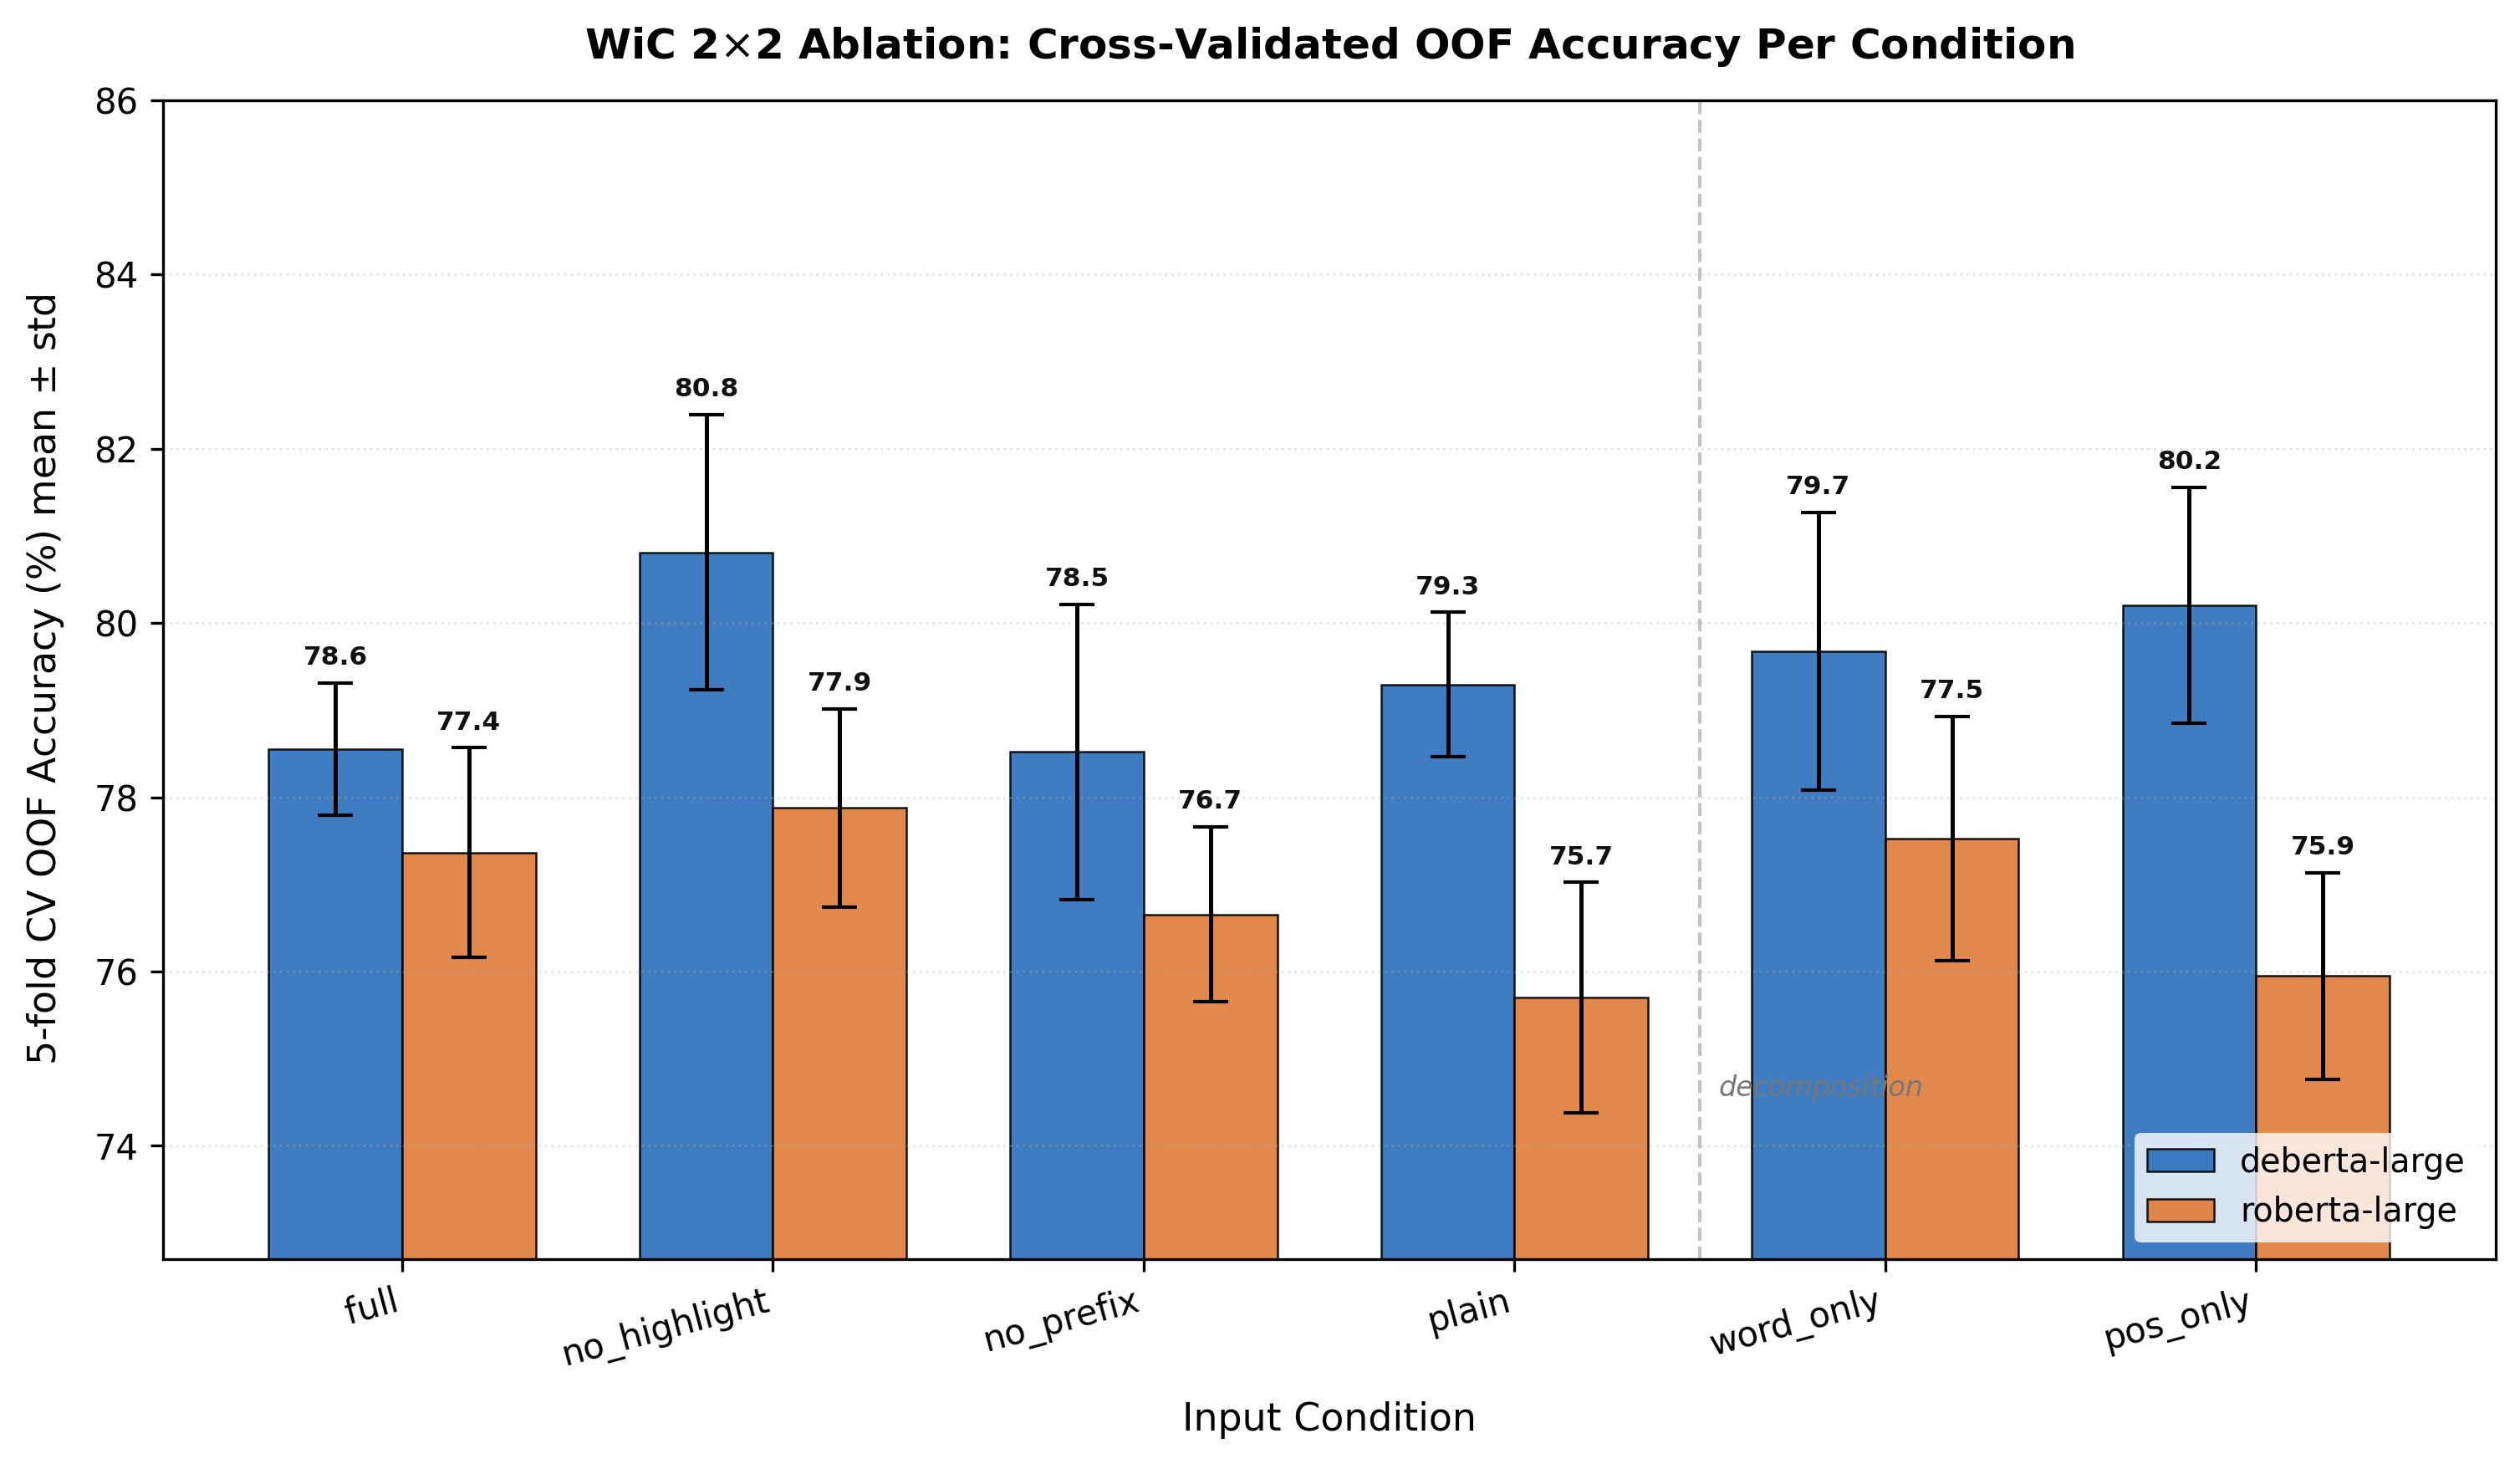
\includegraphics[width=0.86\textwidth]{ablation_plot_cv_300dpi}
\caption{Cross-validated OOF accuracy per input condition (5-fold,
$N = 6066$), mean~$\pm$~std over folds. The dashed vertical line separates the
four core $2 \times 2$ conditions from the two prefix-decomposition conditions.}
\label{fig:cv}
\end{figure}

\subsection{Statistical Analysis of the Contrasts}
\label{subsec:contrasts}

Table~\ref{tab:cv_stats} reports all 7 contrasts per backbone (4 factorial +
3 decomposition). Holm correction is applied to the family of all 7 contrasts
per backbone jointly. Figure~\ref{fig:forest} gives a forest-plot view of the
four core contrasts.

Span highlighting does not improve either backbone and significantly harms
DeBERTa-large. On DeBERTa-large, \texttt{full} vs.\ \texttt{no\_highlight} is
$-2.26$~pp (CI $[-3.20, -1.30]$, $p_{\text{Holm}} < 0.001$): adding the markers
lowers accuracy significantly. On RoBERTa-large the same contrast is $-0.51$~pp
and non-significant. In no setting does highlighting yield a statistically
robust improvement.

The lexical prefix significantly improves both backbones when span markers are
absent. The \texttt{no\_highlight} vs.\ \texttt{plain} contrast (prefix added,
no markers) is positive and significant on both: $+1.52$~pp
(CI $[+0.68, +2.34]$, $p_{\text{Holm}} = 0.003$) on DeBERTa-large and
$+2.18$~pp (CI $[+1.17, +3.15]$, $p_{\text{Holm}} < 0.001$) on RoBERTa-large.
An interaction is also present: the \texttt{full} vs.\ \texttt{no\_prefix}
contrast (prefix with highlighting) is non-significant on both backbones,
suggesting that the markers partly mask the benefit of the prefix. The prefix
is most useful when highlighting is absent.

\begin{figure}[t]
\centering
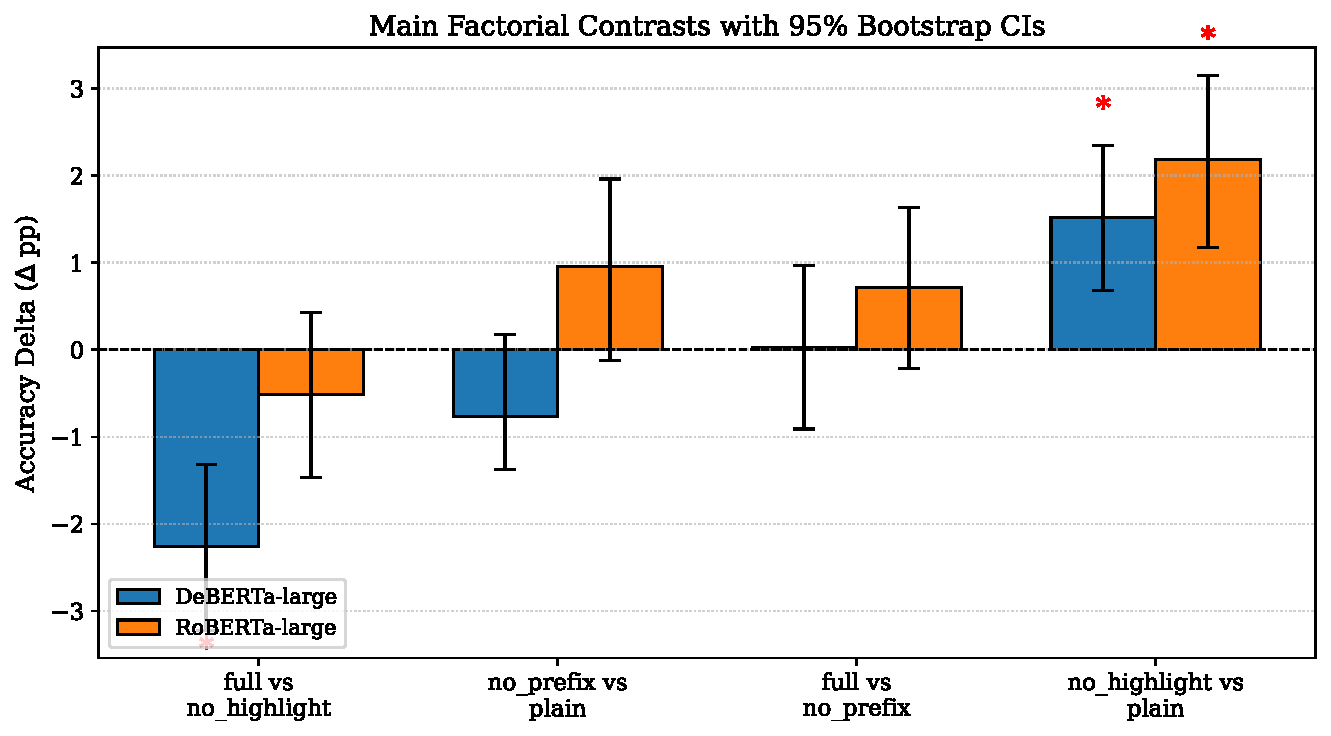
\includegraphics[width=0.68\textwidth]{factorial_contrasts}
\caption{Main factorial contrasts with 95\% bootstrap confidence intervals
(5-fold CV, $N = 6066$). For each contrast, $\Delta = \text{acc}(A) -
\text{acc}(B)$ in percentage points; negative bars indicate that condition $B$
is more accurate. Asterisks mark contrasts that remain significant after
Holm--Bonferroni correction ($p_{\text{Holm}} < 0.05$).}
\label{fig:forest}
\end{figure}

The lemma, not the constant POS tag, drives the prefix effect on RoBERTa-large.
On RoBERTa-large, \texttt{word\_only} vs.\ \texttt{plain} is $+1.83$~pp
($p_{\text{Holm}} = 0.001$); \texttt{pos\_only} vs.\ \texttt{plain} is
$+0.25$~pp (non-significant); \texttt{word\_only} vs.\ \texttt{pos\_only} is
$+1.58$~pp ($p_{\text{Holm}} = 0.006$). Since the POS tag is a constant
(\emph{noun}), this is the expected pattern of a negative control: the lemma
carries the signal and the constant tag does not. These RoBERTa-large decomposition contrasts are listed in
Table~\ref{tab:cv_stats}.
On DeBERTa-large no decomposition contrast reaches significance after Holm
correction; in particular \texttt{pos\_only} has a numerically higher delta than
\texttt{word\_only} on that backbone ($+0.91$ vs.\ $+0.38$~pp), which prevents a
definitive claim. We therefore state the lemma finding as confirmed on
RoBERTa-large only.

\begin{table}[t]
\centering
\caption{Cross-validated contrasts (5-fold, $N = 6066$). Holm correction is
applied to all 7 contrasts per backbone jointly. A checkmark in the Sig.\
column marks $p_{\text{Holm}} < 0.05$.}
\label{tab:cv_stats}
\footnotesize
\begin{tabular}{llcccc}
\toprule
Backbone & Contrast & $\Delta$ Acc.\ (pp) & 95\% CI (pp) & $p_{\text{Holm}}$ & Sig.\\
\midrule
\multirow{7}{*}{DeBERTa-large}
 & \texttt{full} vs.\ \texttt{no\_highlight} & $-2.26$ & $[-3.20, -1.30]$ & $<0.001$ & $\checkmark$\\
 & \texttt{no\_prefix} vs.\ \texttt{plain}   & $-0.77$ & $[-1.71, +0.16]$ & $0.456$ & \\
 & \texttt{full} vs.\ \texttt{no\_prefix}    & $+0.03$ & $[-0.91, +0.97]$ & $0.972$ & \\
 & \texttt{no\_highlight} vs.\ \texttt{plain}& $+1.52$ & $[+0.68, +2.34]$ & $0.003$ & $\checkmark$\\
 & \texttt{word\_only} vs.\ \texttt{plain}   & $+0.38$ & $[-0.46, +1.24]$ & $0.808$ & \\
 & \texttt{pos\_only} vs.\ \texttt{plain}    & $+0.91$ & $[+0.10, +1.71]$ & $0.159$ & \\
 & \texttt{word\_only} vs.\ \texttt{pos\_only}& $-0.53$ & $[-1.35, +0.33]$ & $0.706$ & \\
\midrule
\multirow{7}{*}{RoBERTa-large}
 & \texttt{full} vs.\ \texttt{no\_highlight} & $-0.51$ & $[-1.45, +0.45]$ & $0.602$ & \\
 & \texttt{no\_prefix} vs.\ \texttt{plain}   & $+0.96$ & $[-0.12, +1.96]$ & $0.308$ & \\
 & \texttt{full} vs.\ \texttt{no\_prefix}    & $+0.71$ & $[-0.21, +1.63]$ & $0.419$ & \\
 & \texttt{no\_highlight} vs.\ \texttt{plain}& $+2.18$ & $[+1.17, +3.15]$ & $<0.001$ & $\checkmark$\\
 & \texttt{word\_only} vs.\ \texttt{plain}   & $+1.83$ & $[+0.86, +2.77]$ & $0.001$ & $\checkmark$\\
 & \texttt{pos\_only} vs.\ \texttt{plain}    & $+0.25$ & $[-0.66, +1.17]$ & $0.619$ & \\
 & \texttt{word\_only} vs.\ \texttt{pos\_only}& $+1.58$ & $[+0.61, +2.51]$ & $0.006$ & $\checkmark$\\
\bottomrule
\end{tabular}
\end{table}

The 5-fold CV pools the official training and development splits and
re-partitions them at random; because WiC reuses sentences and target words
across examples, absolute OOF accuracy is not directly comparable to the
official development or test sets, nor to leaderboard figures such as
SenseBERT's $72.1\%$ test accuracy~\cite{levine2020sensebert}. For this reason we
make no claim of leaderboard positioning and rely throughout on the within-fold
paired contrasts, which remain valid since any distribution effect applies
equally to all conditions on each fold.

For orientation, published accuracies on the official WiC test set place the
BERT baseline of the SuperGLUE paper at $69.5\%$ and the human estimate at
$80.0\%$~\cite{wang2019superglue}, with SenseBERT at
$72.1\%$~\cite{levine2020sensebert}. We deliberately do not tabulate our own
accuracies alongside them, since the two quantities are computed on different
data under different protocols. They do, however, indicate the regime at stake:
the $7.9$~pp separating the strongest of these systems from human performance is
the headroom an input-side intervention competes for, and the $2.26$~pp
degradation caused by span markers consumes more than a quarter of it, in the
wrong direction.

\subsection{Error Analysis}
\label{subsec:error}

To understand \emph{how} span highlighting changes predictions, rather than only
its effect on aggregate accuracy, we examine the primary contrast on
DeBERTa-large, \texttt{full} vs.\ \texttt{no\_highlight}, at the level of
individual out-of-fold predictions. Table~\ref{tab:agreement} reports the
agreement between the two conditions over the $N = 6066$ pooled examples.

\begin{table}[t]
\centering
\caption{Prediction agreement between \texttt{full} and \texttt{no\_highlight}
on DeBERTa-large (5-fold OOF, $N = 6066$). \emph{Recovered} examples are
classified correctly by \texttt{no\_highlight} but not by \texttt{full};
\emph{lost} examples are the opposite.}
\label{tab:agreement}
\begin{tabular}{lcc}
\toprule
 & \texttt{no\_highlight} correct & \texttt{no\_highlight} wrong\\
\midrule
\texttt{full} correct & $4398$ & $367$ \;(lost)\\
\texttt{full} wrong   & $504$ \;(recovered) & $797$\\
\bottomrule
\end{tabular}
\end{table}

Removing the markers recovers $504$ examples while losing $367$, a net gain of
$137$ correct predictions. This net difference corresponds exactly to the
$+2.26$~pp out-of-fold gap reported in Section~\ref{subsec:contrasts}
(Table~\ref{tab:cv_stats}): the headline effect is the residual of two sizable,
partially offsetting flows rather than a uniform shift.

We then tested whether the recovered and lost cases differ along simple,
interpretable dimensions: we binned the relative position of the target word in
each sentence as early, middle, or late, and flagged examples in which the
target form occurs more than once. Neither feature separates the two groups: the
position distributions are close (for instance, recovered cases have an
early-position target in the first sentence $56.0\%$ of the time against
$50.1\%$ for lost cases, with no comparable gap in the second sentence), and
target repetition is negligible in both groups (below $1\%$). The effect of the
markers is therefore diffuse rather than concentrated on an identifiable subset
of examples.

Qualitatively, the discordant cases are ordinary polysemy pairs in both
directions. A representative recovered example is \emph{Roll out the paper.}\
vs.\ \emph{The drawer rolled open.}\ (gold label: different senses), which
\texttt{no\_highlight} separates correctly and \texttt{full} does not; lost
cases are of the same nature in the opposite direction. We did not identify a
consistent linguistic property distinguishing when the markers help from when
they hurt; this absence is itself informative, consistent with the special
tokens perturbing the representation broadly rather than interfering with a
specific phenomenon.

% =====================================================================
\section{Discussion}
\label{sec:discussion}

The results challenge the intuitive assumption that explicitly marking the
target word improves WiC: span highlighting yields no benefit on either backbone
and significantly degrades DeBERTa-large. A plausible explanation concerns the
nature of the signals. Span highlighting introduces special tokens absent from
pre-training, initialized from scratch and learned on a small dataset; the
lexical prefix instead reuses in-vocabulary tokens and provides an explicit
lexical anchor. This reading is consistent with evidence from relation
extraction, where Zhou and Chen~\cite{zhou2022improved} report that markers
built from in-vocabulary punctuation can match or outperform markers that
introduce new special tokens. Our results extend this observation to the WiC
cross-encoder setting and quantify it with statistical control.

The decomposition sharpens this picture on RoBERTa-large. Since the SuperGLUE
WiC release exposes no POS field, \texttt{pos\_only} is a constant prefix acting
as a negative control: it does not improve over \texttt{plain}, while
\texttt{word\_only} does and significantly outperforms \texttt{pos\_only},
confirming that the benefit is lexical rather than an artifact of prepending any
token. This is non-trivial given that WiC is known to carry a strong context
bias~\cite{liu2021context}, under which a target-side cue is not guaranteed to
help. On DeBERTa-large the decomposition is
inconclusive---\texttt{pos\_only} numerically exceeds \texttt{word\_only}, though
neither contrast is significant---consistent with the encoder benefiting from any
short prefix as a position cue, largely independent of its lexical content;
separating this from a genuine part-of-speech effect would require the populated
POS field the release lacks. An interaction reinforces the picture: the prefix
helps most when highlighting is absent, suggesting the markers can interfere with
the lexical anchor.

The error analysis in Section~\ref{subsec:error} both sharpens and bounds this
interpretation. The $2.26$~pp out-of-fold advantage of \texttt{no\_highlight} is
not a uniform improvement: removing the markers changes the prediction on
roughly $14\%$ of examples ($504$ recovered and $367$ lost), and the reported
figure is the net of these two flows. Crucially, the recovered and lost subsets
are not separable by target position or by repetition of the target form, and we
could not isolate a linguistic regime in which the markers are systematically
harmful. This is consistent with the mechanism we propose: the out-of-vocabulary
markers, initialized from scratch and learned on a small dataset, perturb
DeBERTa-large's disentangled content--position attention broadly rather than
disrupting a localized phenomenon. It also tempers
any stronger reading: because the change is diffuse and partially
self-cancelling, we characterise span highlighting as a net liability for this
backbone, not as a targeted failure mode.

This interpretation is deliberately cautious: we have not analysed attention
maps or conducted causal interventions, so we do not claim that the model
literally looks at the prefix. A feature-attribution analysis quantifying which
input regions drive the prediction would complement the accuracy-based evidence
reported here, and is planned as a next step.

% =====================================================================
\section{Limitations}
\label{sec:limitations}

No official test-set score was obtainable, as no active official submission
route was available to us at the time of writing. The hyperparameters were tuned on DeBERTa-large and transferred to
RoBERTa-large; within-backbone contrasts are valid, but absolute cross-backbone
comparisons are not principled. The SuperGLUE WiC release exposes no POS field
(verified across all 7{,}466 records), so we could not assess a genuine
lexico-syntactic prefix; testing a real POS signal would require the original
WiC distribution, which encodes a noun/verb distinction, or an external tagger.
Relatedly, the design does not separate whether the benefit of the prefix arises
from improved target localization, from easier optimization during fine-tuning,
or from both. Checkpoint selection is based on held-out-fold accuracy, which may
introduce a small optimistic bias on absolute OOF accuracy; the paired
within-fold contrasts are much less exposed, since the same strategy applies
identically to all conditions in each fold. Finally, the study covers only two encoder
backbones, both used in a
cross-encoder configuration; whether the same input-formatting effects hold for
bi-encoder architectures---such as the one used by
XL-LEXEME~\cite{cassotti2023xllexeme}, where each context is encoded
independently---remains an open question.

% =====================================================================
\section{Conclusion and Future Work}
\label{sec:conclusion}

We presented a controlled ablation of span highlighting and a lexical prefix for
the Word-in-Context task, together with a prefix decomposition. Across a 5-fold
cross-validation on two large encoders ($N = 6066$), span highlighting provided
no benefit and significantly degraded DeBERTa-large, while the lexical prefix
significantly improved both backbones when markers are absent; on RoBERTa-large
the lemma, not the constant POS tag, is the active component, and the
degradation caused by markers is diffuse rather than localized. The contribution
is methodological: statistically grounded evidence on input-design choices often
treated as implementation details.

Several directions remain open: submitting to the official test set once the
platform is restored, and training on the full labelled pool (train + dev) as is
standard after cross-validation; moving beyond passive marking by emphasizing
the span through token-weighted losses or an attention bias, and re-initializing
the \texttt{<TW>}/\texttt{</TW>} embeddings from existing vocabulary tokens to
test whether cold-start initialization is the source of the degradation; using
the POS annotation of the original WiC distribution, or an external tagger, to
assess a genuine lexico-syntactic prefix; extending to other tasks such as
named-entity recognition; and including
DeBERTa-v3~\cite{he2023debertav3} to test whether the results generalize beyond
masked-language-modeling pre-training.

\begin{credits}
\subsubsection{\ackname} The authors thank the supervisors and academic staff
involved in the refinement of this work.

\subsubsection{\discintname} The authors have no competing interests to declare
that are relevant to the content of this article.
\end{credits}

% =====================================================================
\begin{thebibliography}{99}

\bibitem{pilehvar2019wic}
Pilehvar, M.T., Camacho-Collados, J.: WiC: the word-in-context dataset for
evaluating context-sensitive meaning representations. In: Proc.\ NAACL-HLT 2019,
pp.\ 1267--1273 (2019). \url{https://doi.org/10.18653/v1/N19-1128}

\bibitem{wang2019superglue}
Wang, A., Pruksachatkun, Y., Nangia, N., Singh, A., Michael, J., Hill, F.,
Levy, O., Bowman, S.R.: SuperGLUE: a stickier benchmark for general-purpose
language understanding systems. In: Advances in NeurIPS 32, pp.\ 3261--3275
(2019)

\bibitem{devlin2019bert}
Devlin, J., Chang, M.W., Lee, K., Toutanova, K.: BERT: pre-training of deep
bidirectional transformers for language understanding. In: Proc.\ NAACL-HLT
2019, pp.\ 4171--4186 (2019). \url{https://doi.org/10.18653/v1/N19-1423}

\bibitem{liu2019roberta}
Liu, Y., Ott, M., Goyal, N., Du, J., Joshi, M., Chen, D., Levy, O., Lewis, M.,
Zettlemoyer, L., Stoyanov, V.: RoBERTa: a robustly optimized BERT pretraining
approach. arXiv:1907.11692 (2019)

\bibitem{he2021deberta}
He, P., Liu, X., Gao, J., Chen, W.: DeBERTa: decoding-enhanced BERT with
disentangled attention. In: International Conference on Learning Representations
(ICLR) (2021)

\bibitem{he2023debertav3}
He, P., Gao, J., Chen, W.: DeBERTaV3: improving DeBERTa using ELECTRA-style
pre-training with gradient-disentangled embedding sharing. In: International
Conference on Learning Representations (ICLR) (2023). arXiv:2111.09543

\bibitem{levine2020sensebert}
Levine, Y., Lenz, B., Dagan, O., Ram, O., Padnos, D., Sharir, O.,
Shalev-Shwartz, S., Shashua, A., Shoham, Y.: SenseBERT: driving some sense into
BERT. In: Proc.\ ACL 2020, pp.\ 4656--4667 (2020).
\url{https://doi.org/10.18653/v1/2020.acl-main.423}

\bibitem{soares2019matching}
Baldini Soares, L., FitzGerald, N., Ling, J., Kwiatkowski, T.: Matching the
blanks: distributional similarity for relation learning. In: Proc.\ ACL 2019,
pp.\ 2895--2905 (2019). \url{https://doi.org/10.18653/v1/P19-1279}

\bibitem{cassotti2023xllexeme}
Cassotti, P., Siciliani, L., De Gemmis, M., Semeraro, G., Basile, P.:
XL-LEXEME: WiC pretrained model for cross-lingual lexical semantic change. In:
Proc.\ ACL 2023 (Short Papers), pp.\ 1577--1585 (2023).
\url{https://doi.org/10.18653/v1/2023.acl-short.135}

\bibitem{martelli2021mclwic}
Martelli, F., Kalach, N., Tola, G., Navigli, R.: SemEval-2021 task 2:
multilingual and cross-lingual word-in-context disambiguation (MCL-WiC). In:
Proc.\ SemEval-2021, pp.\ 24--36 (2021).
\url{https://doi.org/10.18653/v1/2021.semeval-1.3}

\bibitem{gupta2021mcliitk}
Gupta, R., Mundra, J., Mahajan, D., Modi, A.: MCL@IITK at SemEval-2021 task 2:
multilingual and cross-lingual word-in-context disambiguation using augmented
data, signals, and transformers. In: Proc.\ SemEval-2021, pp.\ 511--520 (2021).
\url{https://doi.org/10.18653/v1/2021.semeval-1.62}

\bibitem{zhou2022improved}
Zhou, W., Chen, M.: An improved baseline for sentence-level relation extraction.
In: Proc.\ AACL-IJCNLP 2022 (Short Papers), pp.\ 161--168 (2022)

\bibitem{huang2019glossbert}
Huang, L., Sun, C., Qiu, X., Huang, X.: GlossBERT: BERT for word sense
disambiguation with gloss knowledge. In: Proc.\ EMNLP-IJCNLP 2019,
pp.\ 3507--3512 (2019). \url{https://doi.org/10.18653/v1/D19-1355}

\bibitem{firth1957synopsis}
Firth, J.R.: A synopsis of linguistic theory, 1930--1955. In: Studies in
Linguistic Analysis, pp.\ 1--32. Blackwell, Oxford (1957)

\bibitem{akiba2019optuna}
Akiba, T., Sano, S., Yanase, T., Ohta, T., Koyama, M.: Optuna: a next-generation
hyperparameter optimization framework. In: Proc.\ 25th ACM SIGKDD International
Conference on Knowledge Discovery and Data Mining, pp.\ 2623--2631 (2019).
\url{https://optuna.org}

\bibitem{liu2021context}
Liu, Q., McCarthy, D., Korhonen, A.: Measuring context-word biases in lexical
semantic datasets. arXiv:2112.06733 (2021)

\end{thebibliography}

\end{document}
